\documentclass[english, DIV=calc, BCOR=5mm, fontsize=11pt, portrait]{scrartcl}	 % A4 paper and 11pt font size

\usepackage[T1]{fontenc}
\usepackage[utf8]{inputenc}
\usepackage[ngerman,english]{babel} % English language/hyphenation
\usepackage[protrusion=true,expansion=true]{microtype} % Better typography
\usepackage{amsmath,amsfonts,amsthm} % Math packages
\usepackage[svgnames]{xcolor} % Enabling colors by their 'svgnames'
\usepackage[hang, small,labelfont=bf,up,textfont=it,up]{caption} % Custom captions under/above floats in tables or figures
\usepackage{booktabs} % Horizontal rules in tables
\usepackage{fix-cm}	 % Custom font sizes - used for the initial letter in the document
\usepackage{setspace}
\usepackage{hyperref}
\usepackage{graphicx}
\usepackage{tikz}
\usepackage[top=3cm,bottom=3cm]{geometry}
\usepackage{longtable}
\usepackage{pdflscape}
\usepackage[style=american]{csquotes}
\usepackage{here} 

%\usepackage{sectsty} % Enables custom section titles
%\allsectionsfont{\usefont{OT1}{phv}{b}{n}} % Change the font of all section commands

\usepackage{fancyhdr} % Needed to define custom headers/footers
\pagestyle{fancy} % Enables the custom headers/footers
\usepackage{lastpage} % Used to determine the number of pages in the document (for "Page X of Total")

% Headers - all currently empty
\lhead{English B2}
\chead{Special Purposes Seminar: Freedom on the Internet}
\rhead{Team 3}

% Footers
\lfoot{}
\cfoot{\footnotesize Page \thepage\ of \pageref{LastPage}}
\rfoot{} % "Page 1 of 2"

\renewcommand{\headrulewidth}{0.2pt} % No header rule
\renewcommand{\footrulewidth}{0.4pt} % Thin footer rule

\usepackage{lettrine} % Package to accentuate the first letter of the text
\newcommand{\initial}[1]{ % Defines the command and style for the first letter
\lettrine[lines=3,lhang=0.3,nindent=0em]{
\color{DarkGoldenrod}
{\textsf{#1}}}{}}

%------------------------------------------------------------------------------
%	TITLE SECTION
%------------------------------------------------------------------------------

\usepackage{titling} % Allows custom title configuration

\newcommand{\HorRule}{\color{DarkGoldenrod} \rule{\linewidth}{1pt}} % Defines the gold horizontal rule around the title

\pretitle{ \includegraphics[width=10cm]{./img/logo-transp.png}  \vspace{-4em}
 %\\ \vspace{1cm}
 \hspace{-20em}
\mbox{\textbf{if you are free --- you cannot be free of risk}}
\begin{flushleft} \HorRule \fontsize{50}{50} \usefont{OT1}{phv}{b}{n} \color{DarkRed} \selectfont} % Horizontal rule before the title

\title{Freedom on the Internet} % Your article title

\posttitle{\par\end{flushleft}\vskip 0.5em} % Whitespace under the title

\preauthor{\begin{flushleft}\large \lineskip 0.5em \usefont{OT1}{phv}{b}{sl} \color{DarkRed}} % Author font configuration

\author{David\,(s72838), Maxym\,(s72810), Wolf\,(s72785) } %names

\postauthor{\footnotesize \usefont{OT1}{phv}{m}{sl} \color{Black} \\ % Configuration for the institution name
Dresden University of Applied Sciences % Your institution
\par\end{flushleft}\HorRule} % Horizontal rule after the title

\date{} % Add a date here if you would like one to appear underneath the title block

%Einleitung

%- vid:privacy
%- tor
%- Bitcoin
%- Stellar

%Handout

\begin{document}

%bild

% Print the title
\maketitle

\tableofcontents
%	\section{}%- deckblatt, team, bild;
%if you are free
%you cannot be free of risk

\newpage
	
\section{Abstract}%- abstract (we abschaffen, quellen indirekt einbringen)

%\begin{multicols}{2}{
% include...
%}

\begin{onehalfspace}

\initial{S}ince summer 2013 the world is aware of illegal surveillance by \textit{state agencies} around the world violating fundamental human and civil rights justified by \textit{false claims} like child protection, copyright, drug policy and fighting terrorism.
Besides we all pay for this folly, most companies and individuals act just according to their financial interests.
No doubt \textit{money is the main incentive} for criminals as well as for corporations that control politicians nowadays.
In January 2009 a new kind of money was launched.
The network is the currency, transparent, pseudonymous, not eligible to direct regulation by banks nor governments. Remaining controversial it enables freedom and international transactions.
The Electronic Frontier Foundation started even earlier to implement an anonymity network: tor - the onion routing.
Our teams researched on the nets discovered that inventors built asymmetric cryptography with the most durable methods found at that time.
\textit{Blockchain technology} for the first time in history \textit{manages to solve the trust problem}.
Many people do not understand the technical matters or focus on their national currency only. That is why, by teaching about freedom in this seminar rather than the technological background or plain capitalization, the team intends to make a difference and introduce usable technology that enables modern financial computing.
Use cases, that are adopted already by millions of users who care for their privacy and civil rights, will be presented.
The first sources were texts that introduce the tor network.
The seminar is based on the scheme behind Bitcoin as described in the key paper by Satoshi Nakamoto. Moreover, a glance at the more accessible approach provided by Stellar in publications by the non-commercial company behind is taken.
\textit{Cryptography is no crime}. There can be \textit{no freedom without risk and responsibility}.
Now it is just the \textit{owners holding} the vital \textit{key} to control.
\end{onehalfspace}

\newpage 

%\end{multicols}

\section{Glossary}%- glossary (10)

\begin{longtable}{p{3cm}||p{3cm}|p{3cm}|p{4cm}}
%\caption{Glossary}
Word/Collocation \newline
Word Family Examples \newline
Word Types &
Translation &
Definition or \newline
Synonym &
Sentence Example \\
\endhead
\hline
\hline
\textbf{peer-to-peer network} (noun)	& Teilnehmer-Netzwerk			& network of equitable parties					& file sharing is usually done on \textbf{peer-to-peer network}s	\\
\hline
\textbf{digital signature} (noun)		& Digitale Unterschrift			& signature added to a digital document so it can be verified which person signed	& the ability to manage public keys for verifying \textbf{digital signature}s provides each e-mail user the individual power to control who communicates with her and can therefore completely eliminate the practice of spamming	\\
\hline
\textbf{hash} (noun)				& Streu\-sum\-me					& identifier, cryptographic single way fucntion	& it is not easily possible to calculate the origin of a \textbf{hash} 	\\
\hline
\textbf{node} (noun)				& Netzknoten					& point in a network or diagram at which lines or pathways intersect or branch	& the intersections of two or more such arteries would clearly become major \textbf{nodes} of traffic and urban activity	\\
\hline
\textbf{best effort} (noun)		& größte Anstrengung			& the best that can be done unter certain limitations	& this is done on a \textbf{best effort} basis	\\
\hline
\textbf{inherent} (adj.)			& innewohnend, anhaftend		& something as a permanent, essential, or characteristic attribute	& any form of mountaineering has its \textbf{inherent} dangers	\\
\hline
%david
\textbf{surveillance} (noun)	\newline survey (noun) \newline surveillance camera (collocation) \newline survey (verb) & Überwachung	& the act of carefully watching a person suspected of a crime & The police are keeping the suspects under constant \textbf{surveillance} \\
\hline
\textbf{revelation} (noun) \newline reveal (verb) \newline revealable (adjective) \newline Book of Revelation (collocation) & Enthüllung & the act of making people aware of something that has been secret & since \textbf{revelation}s about the surveillance strategies of US and UK spies, Tor has become a focus of criticism \\
\hline
\textbf{evading} (verb) \newline evaded (adjective) \newline evading from supervision (noun) \newline evade tax (collocation) & umgehen, ausweichen & to find a way of not doing something & users \textbf{evading} censorship in certain parts of the world \\
\hline
\textbf{prying} (adjective) \newline pry about (collocation) \newline pry (verb) \newline prying effect (noun) & neugierig & to try to find out private facts about a person & The fact that those requiring anonymity are extremely mindful of the \textbf{prying} eyes of authorities was reiterated last night as details emerged of the 29-year-old that blew the whistle on the US surveillance \\
\end{longtable}

\section{MindMap}

\includegraphics[width=13cm]{./img/MindMap.pdf}

\section{Exercises}

\subsection{Word Puzzle}

Find the following English terms in the Word-Puzzle
below. The words can be hidden in a vertical,
horizontal, and diagonal way as well as forward and
backward. Also try to translate the words into
German.
\vspace{0.5cm}
\begin{figure}[H]
	\begin{minipage}{6cm}
		\begin{enumerate}
		\item CANDID 
		\item DISGUISE 
		\item EMPHASIS 
		\item FACILITATING 
		\item LAYERS
		\end{enumerate}
	\end{minipage}
	%\hfill
	\begin{minipage}{6cm}
		\begin{enumerate}
		\setcounter{enumi}{5}
		\item OBSCURES
		\item PROLIFERATION
		\item PRYING
		\item SOPHISTICATED
		\item SURVEILLANCE
		\end{enumerate}
	\end{minipage}
	\\ \vspace{0.5cm} \\
	\begin{minipage}{13cm}
		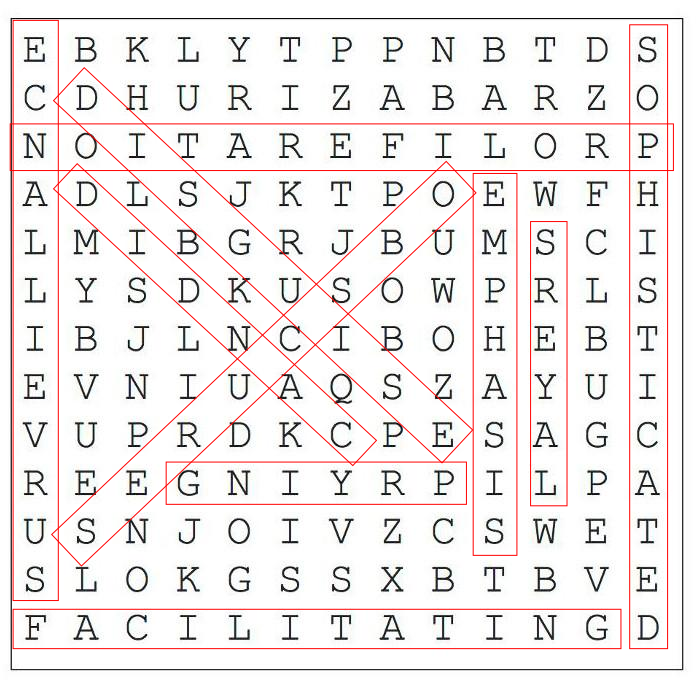
\includegraphics[width=13cm]{./img/Exercise_-_Word_Puzzle_crop.jpg}
	\end{minipage}
\end{figure}

\newpage 

\subsection{Bitcoin Transfer}

Trade goods for Bitcoin by offering a transaction for signature and track the transactions in the public chain by noting your transaction-id.
Take this as an imaginary task and discuss what you would buy without revealing your identity.

\begin{figure}[H]
	\begin{minipage}{4.5cm}
		\begin{itemize}
		\item txid
		\item timestamp(s)
		\end{itemize}
	\end{minipage}
	\begin{minipage}{4.5cm}
		\begin{itemize}
		\item payee(s)
		\item payer(s)
		\end{itemize}
	\end{minipage}
	\begin{minipage}{4.5cm}
		\begin{itemize}
		\item amount(s)
		\item signature(s)
		\end{itemize}
	\end{minipage}
\end{figure}

\subsection{Crossword}

\begin{figure}[H]
	\begin{minipage}{9cm}
		\includegraphics[width=9cm]{./img/cw-stellar.png}
	\end{minipage}
	\hfill
	\begin{minipage}{6cm}
		\begin{enumerate}
		\item Mittel,Gelder
		\item dezentralisiert 
		\item Umwandlung
		\item passend, entsprechend
		\item Währung 
		\item etwas mieten 
		\item eine Taktik
		\item jmd. beauftragen
		\item anfragen
		\end{enumerate}
	\end{minipage}
\end{figure}

\section{Discussion}
	
\begin{enumerate}
\item Do you use tor? When you would, for what?
\item Would you have a use case for Bitcoin?
\item What are drawback in adoptions like Stellar?	
\end{enumerate}

\newpage

\section{Bibliography (\href{http://www2.liu.edu/cwis/cwp/library/workshop/citmla.htm}{MLA})}


\begin{description}
%david
	\item[tor1:] \hfill \\
		Philby, Charlotte.
		\href{http://www.independent.co.uk/news/media/online/the-tor-system-welcome-to-the-dark-internet-where-you-can-search-in-secret-8651364.html}{\enquote{The Tor 	System: Welcome to the Dark Internet Where You Can Search in Secret.}}
		%\url{http://www.independent.co.uk/news/media/online/the-tor-system-welcome-to-the-dark-internet-where-you-can-search-in-secret-8651364.html}
		\emph{The Independent}.
		Independent Digital News and Media, 10\,June\,2013.
		Web.~28\,Apr.\,2015.
	\item[tor2:] \hfill \\
		Dredge, Stuart.
		\href{http://www.theguardian.com/technology/2013/nov/05/tor-beginners-guide-nsa-browser}{\enquote{What Is Tor? A Beginner's Guide to the Privacy Tool.}}
		%\url{http://www.theguardian.com/technology/2013/nov/05/tor-beginners-guide-nsa-browser}
		\emph{theguardian}, 5\,Nov.\,2013.
		Web.~27\,Apr.\,2015.
%wolf
	\item[Bitcoin:]\hfill \\
		Nakamoto, Satoshi.
		\href{http://bitcoin.org/bitcoin.pdf}{\enquote{Bitcoin: A Peer-to-Peer Electronic Cash System.}}
		%\url{http://bitcoin.org/bitcoin.pdf}. \\
		\href{http://www.metzdowd.com/mailman/listinfo/cryptography}{\emph{The Cryptography Mailing List}}, 31\,Oct.\,2008.
		Web.~1\,May\,2015.
%maxym
	\item[Stellar1:] \hfill \\
		Stellar Team.
		\href{https://www.stellar.org/blog/introducing-stellar}{\enquote{Introducing Stellar.}} 
		%\url{https://www.stellar.org/blog/introducing-stellar}
		\emph{Web log post}.
		Stellar, 31\,July\,2014.
		Web.~26\,Apr.\,2015.
	\item[Stellar2:] \hfill \\
		Stellar Team.
		\href{http://thenextweb.com/insider/2014/08/01/stellar-open-source-solution-international-money-transfers-currency}{\enquote{What You Need to Know About 	Stellar's New Currency.}}
		%\url{http://thenextweb.com/insider/2014/08/01/stellar-open-source-solution-international-money-transfers-currency}
		\emph{TNW Network All Stories RSS}, 31\,July\,2014.
		Web.~26\,Apr.\,2015.
%videos wolf
	\item[Video:Privacy] \hfill \\
		laquadrature.net.
		\href{https://mediakit.laquadrature.net/view.php?id=1302}{\enquote{LQDN-privacy-201402.mov}}
		%\url{https://mediakit.laquadrature.net/view.php?id=1302}
		\emph{La Quadrature Du Net, Mediatkit}, 11\,Feb\,2014.
		Web.~1\,May\,2015.
	\item[Video:Bitcoin] \hfill \\
		We Use Coins project.
		\href{http://youtu.be/Gc2en3nHxA4}{\enquote{What is Bitcoin? (v2)}}
		%\url{http://youtu.be/Gc2en3nHxA4}
		%\url{https://www.weusecoins.com/}
		\emph{We Use Coins dot com, Frontpage}, 24\,Apr.\,2014.
		Web.~1\,May\,2015.

\end{description}

\end{document}
